
Sia per l'analisi delle potenzialit� del magazzino sia per la ricerca dell'insieme di set pi� conveniente per colmare il gap per raggiungere un determinato obiettivo, si utilizza l'algoritmo della ricorsione. Si � quindi ritenuto utile valutare i tempi di esecuzione per un caso di studio semplice, ma indicativo della crescita esponenziale della complessit� del problema.

\section{Caso di studio}

Si suppone di partire da un magazzino vuoto e acquistare i seguenti tre set della serie Creator Export:
\begin{itemize}
\item Fiat 500 (10271-1)
\item London Bus (10258-1)
\item NASA Apollo 11 (10266-1)
\end{itemize}
Dopodich� si calcolano le sequenze di set che si possono costruire cambiando la percentuale di completamento a ogni prova. Si ottengono i risultati di seguito riportati nella tabella \ref{TAB:tempi_ricorsione} e nel grafico \ref{FIG:tempi_ricorsione}.
Si osserva come nel momento in cui la percentuale di completamento dei set scende sotto un valore sufficientemente basso a seconda della disponibilit� di pezzi in magazzino, i tempi aumentano in quanto il numero di soluzioni parziali valide aumenta considerevolmente.

\newpage

\vspace{0.5cm}
\begin{table}[htbp]
\begin{center}
\begin{tabular}{||c|c||}
\hline
{\bfseries percentuale di completamento dei set} & {\bfseries tempi in secondi}\\
\hline
\hline
90\% & 0.15\\
80\% & 0.15\\
70\% & 0.15\\
60\% & 0.15\\
50\% & 0.15\\
25\% & 30\\
20\% & 20\\
\hline
\hline
\hline
\end{tabular}
\caption {\label{TAB:tempi_ricorsione}  Tempi di esecuzione dell'algoritmo di ricorsione per diverse percentuali di completamento dei set}
\end{center}
\end{table}
\vspace{0.5cm}


\begin{figure}[htbp]
    \centering
    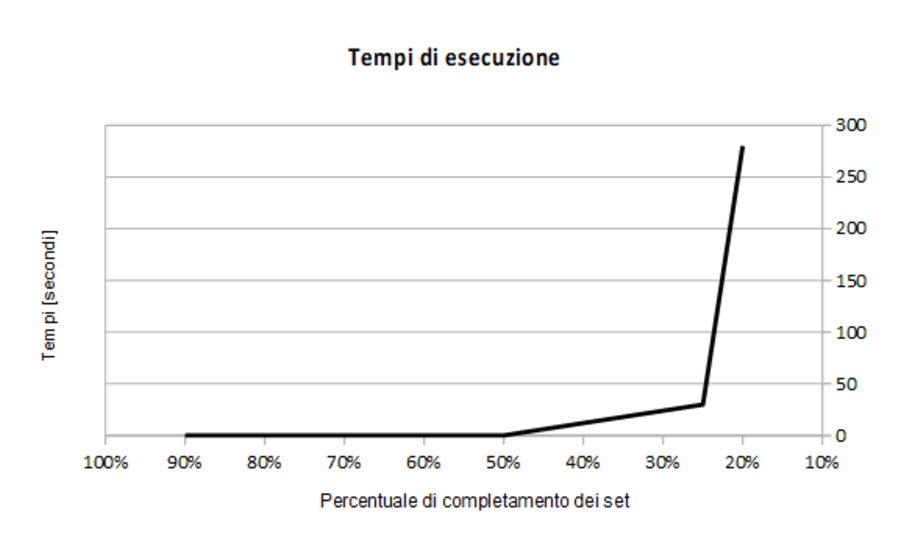
\includegraphics[scale=0.95]{risultati_sperimentali/tempi_ricorsione.eps}
\vspace{-5pt} \caption{Tempi dell'algoritmo di ricorsione}
\label{FIG:tempi_ricorsione}
\end{figure}
\vspace{0.5cm}

